\documentclass[12pt, a4paper]{article}

\usepackage[paper=a4paper, left=1.5cm, right=1.5cm, bottom=2cm, 		top=2cm]{geometry}
\usepackage[utf8]{inputenc}
\usepackage[T1]{fontenc}
\usepackage{interfaz}
\usepackage{caratula}
\newcommand{\comment}[1]{}
%\usepackage[spanish]{babel}
%\selectlanguage{spanish} 
\usepackage{algorithm2e} %for psuedo code
\usepackage{amsmath}
\usepackage{amsfonts}
\usepackage{graphicx}
\usepackage[colorlinks,citecolor=black,filecolor=black,linkcolor=black,    urlcolor=black]{hyperref}
\setcounter{secnumdepth}{5}
\setcounter{tocdepth}{5}
\SetKwIF{If}{ElseIf}{Else}{si}{entonces}{sin\'o, si}{de lo contrario}{fin si}
\SetKwFor{While}{Mientras}{hacer}{fin ciclo}%
\SetKwFor{For}{Para cada}{hacer}{fin para}%
\usepackage{mathtools}
\DeclarePairedDelimiter{\ceil}{\lceil}{\rceil}
\SetKwProg{Fn}{función}{}{fin función}%

\titulo{Trabajo Pr\'actico 1}

\materia{Bases de datos}
\grupo{Grupo 7}
\integrante{Lavia, Alejandro}{43/11}{lavia.alejandro@gmail.com}
\integrante{, Jorge}{}{}
\integrante{Rey, Esteban}{657/10}{estebanlucianorey@gmail.com}
\integrante{Tripodi, Guido}{843/10}{guido.tripodi@hotmail.com}


\begin{document}

\maketitle
\tableofcontents
\newpage

\newpage
\section{Ejercicio 1} 
\subsection{Descripci\'on de problema}

\begin{verbatim}
symbol(a).
symbol(b).
symbol(c).

% Algunas regex de ejemplo

regexEj(1, a). % a
regexEj(2, or(a, b)). % a|b
regexEj(3, concat(E1, E2)) :- regexEj(1, E1), regexEj(2, E2). % a(a|b)
regexEj(4, star(E2)) :- regexEj(2, E2). % (a|b)*
regexEj(5, or(star(E1), E4)) :- regexEj(1, E1), regexEj(4, E4). % (a*|(a(a|b))*)
regexEj(6, star(or(a, ab))). %(a|ab)*
regexEj(7, concat(or(a, concat(a,b)), or(b, empty))). %(a|ab)(b|)
regexEj(8, concat(star(a), star(b))). %a*b*
regexEj(9, star(or(star(a), star(b)))).


% Ejercicio 1: tieneEstrella(+RegEx)


tieneEstrella(concat(X,_)) :- tieneEstrella(X).
tieneEstrella(concat(_,Y)) :- tieneEstrella(Y).
tieneEstrella(or(X,_)) :- tieneEstrella(X).
tieneEstrella(or(_,Y)) :- tieneEstrella(Y).
tieneEstrella(star(_)).


% Ejercicio 2: longitudMaxima(+RegEx, -Length)

longitudMaxima(empty, 0).
longitudMaxima(Cadena,Long) :- symbol(Cadena), Long is 1.
longitudMaxima(or(X,Y), Long) :- 
    not(tieneEstrella(or(X,Y))), 
    longitudMaxima(X, Long1), 
    longitudMaxima(Y,Long2), 
    Long is max(Long1,Long2).
longitudMaxima(concat(X,Y), Long) :- 
    not(tieneEstrella(concat(X,Y))), 
    longitudMaxima(X, Long1), 
    longitudMaxima(Y, Long2), 
    Long is Long1 + Long2.

% Ejercicio 3: cadena(?Cadena)

cadena([]).
cadena([X | XS]):- cadena(XS), symbol(X).

% Ejercicio 4: match_inst(+Cadena, +RegEx)

match_inst([], empty).
match_inst([X], X) :- symbol(X).
match_inst(Cadena, or(X,_)) :- match_inst(Cadena, X).
match_inst(Cadena, or(_,Y)) :- match_inst(Cadena, Y).
match_inst(Cadena, concat(Y,Z)) :- 
    append(C1, C2, Cadena), 
    match_inst(C1,Y), 
    match_inst(C2, Z).
match_inst([], star(_)). %0 apariciones.
match_inst(Cadena, star(Y)) :- 
    append(C1, C2, Cadena), 
    not(length(C1,0)), 
    match_inst(C1, Y), 
    match_inst(C2, star(Y)).

% Ejercicio 5: match(?Cadena, +RegEx)

match(Cadena, RegEx) :- cadena(Cadena), match_inst(Cadena, RegEx).

% Ejercicio 6: diferencia(?Cadena, +RegEx, +RegEx)

diferencia(Cadena, Exp1, Exp2) :-
    match(Cadena, Exp1), 
    not(match(Cadena,Exp2)).

% Ejercicio 7: prefijoMaximo(?Prefijo, +Cadena, +RegEx)
prefijoMaximo(Prefijo, Cadena, Exp) :- 
    append(Prefijo,_,Cadena), 
    match(Prefijo, Exp), 
    length(Prefijo, T), 
    not(hayPrefijoMayor(Cadena,Exp,T)).

%hayPrefijoMayor(+Cadena, +Exp, +T)
hayPrefijoMayor(Cadena, Exp, T):- 
    append(Prefijo,_,Cadena), 
    length(Prefijo, TI), 
    TI > T, 
    match(Prefijo,Exp).

% Ejercicio 8: reemplazar(+X, +R, +E, Res)

reemplazar([], _, _, []).

%si no tengo un prefijo que matchee, busco en la cola de la cadena.
reemplazar([X | XS], Exp, Sust, [X | Rec]) :- 
    not(prefijoMaximo(_, [X | XS], Exp)), 
    reemplazar(XS, Exp, Sust, Rec).

%Si el prefijo maximo es el vacio, lo saltamos.
reemplazar([X | XS], Exp, Sust, [X | Rec]) :- 
    prefijoMaximo([], [X | XS], Exp), 
    reemplazar(XS, Exp, Sust, Rec).

%Si hay un prefijo maximo bueno.
reemplazar(Cadena, Exp, Sust, Res) :- 
    prefijoMaximo(P, Cadena, Exp), 
    length(P,TamP), 
    TamP > 0, 
    append(P, D, Cadena), 
    reemplazar(D, Exp, Sust, Rec), 
    append(Sust, Rec, Res).


% test_2_Y: longitudMaxima

test_2_Y :- test_2_1, test_2_2, test_2_3.

test_2_1 :- longitudMaxima(or(a, b), T), T == 1.
test_2_2 :- longitudMaxima(concat(concat(concat(a,b),b),a),T), T == 4.
test_2_3 :- longitudMaxima(or(concat(concat(a,b),b),a),T), T == 3.
test_2_4 :- longitudMaxima(or(concat(concat(a,star(b)),b),a),T), T == false.

% test_3_Y: longitudMaxima

test_3_Y :- test_3_1, test_3_2, test_3_3, test_3_4.

test_3_1 :- cadena(C), C == [a,b,c].
test_3_2 :- cadena(C), C == [a,a,a,a,a].
test_3_3 :- cadena(C), C == [a,a,b].
test_3_4 :- cadena(C), C == [a,b,c,a,b].

% test_5_Y: match

test_5_Y :- test_5_1, test_5_2, test_5_3, test_5_4.

test_5_1 :- match(X, star(a)), X == [a,a,a,a].
test_5_2 :- match(X, star(concat(star(a), star(b)))), X == [a, b, b, a, a].
test_5_3 :- match(X, star(or(star(a), star(b)))), X == [b, b].
test_5_4 :- match(X,  or(star(a), star(b))), X = [b,b,b,b,b,b,b].

% test_6_Y: diferencia

test_6_Y :- test_6_1, test_6_2, test_6_3.

test_6_1 :- diferencia(X, star(a), star(b)), X == [a, a, a, a, a, a, a].
test_6_2 :- diferencia(X,concat(a,star(b)),c), X == [a, b, b, b, b, b, b, b, b].
test_6_3 :- diferencia(X,concat(a,or(star(b),a)),c), X == [a, b, b, b, b, b, b, b].

% test_7_Y: prefijoMaximo

test_7_Y :- test_7_1, test_7_2,test_7_3.

test_7_1 :- prefijoMaximo(P, [a,b,a,b,a,b], concat(star(a),star(b))), P == [a,b].
test_7_2 :- prefijoMaximo(P, [a,a,a,b,b,b,b,b,a,b,b,b], concat(star(a),star(b))), P == [a, a, a, b, b, b, b, b].
test_7_3 :- prefijoMaximo(P, [a,a,a,b,b,b,b,b,a,b,b,b], concat(a,star(b))), P == [a].

% test_8_Y: reemplazar

test_8_Y :- test_8_1, test_8_2,test_8_3.

test_8_1 :- reemplazar([a,a,a,b,b,a,b,c],concat(a,star(b)), [1],X), X == [1, 1, 1, 1, c].
test_8_2 :- reemplazar([a,a,a,b,b,a,b,c],or(a,star(b)), [1],X), X == [1, 1, 1, 1, 1, 1, c].
test_8_3 :- reemplazar([a,a,a,b,b,a,b,c],concat(star(a),star(c)), [1],X), X == [1, b, b, 1, b, 1].

all_Test :- test_2_Y,test_3_Y,test_5_Y,test_6_Y, test_7_Y, test_8_Y.

\end{verbatim}
\subsection{Modelo de Entidad Relación y Modelo Relacional derivado}
Se realizo un Modelo de Entidad Relación y Modelo Relacional derivado, los cuales fueron utilizados para implementar la solución. \\

A continuación se muestra el MER realizado:\\

\vspace*{0.3cm} \vspace*{0.3cm}
  \begin{center}
 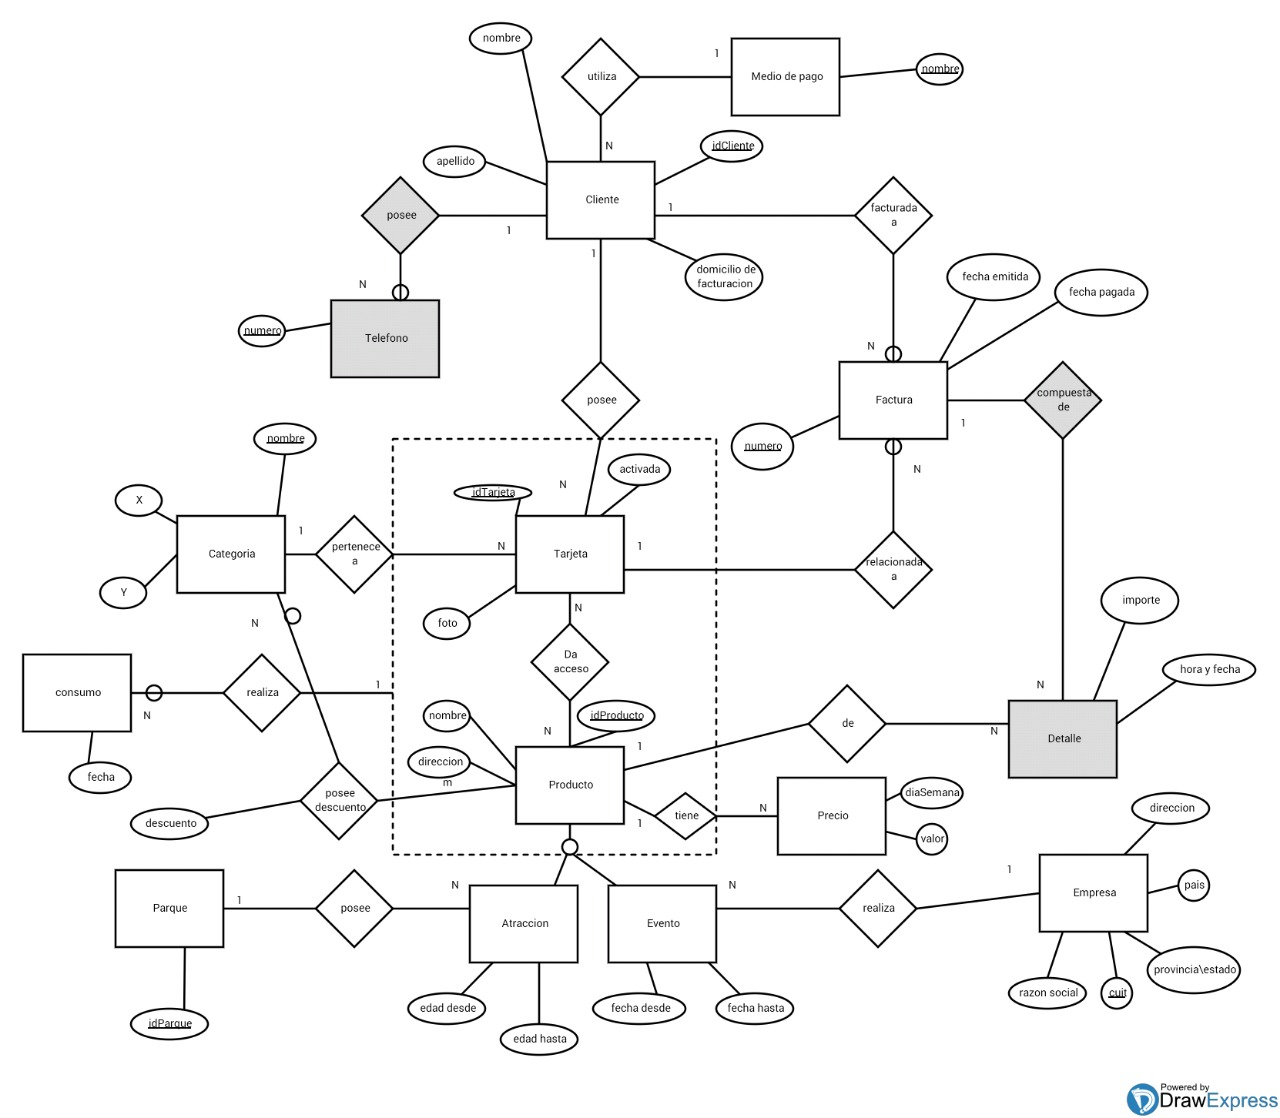
\includegraphics[scale=0.43]{der.jpeg}
 {$Gr$\'a$fico$ $Modelo$ $Entidad$ $Relaci$\'o$n$}
  \end{center}
  \vspace*{0.3cm}
  
En base al MER realizado se derivan las siguientes tablas con sus respectivos atributos y claves:\\

\textbf{Cliente}(\underline{idCliente}, nombre, apellido, domicilioFact)\\
PK =  $\lbrace$idCliente$\rbrace$  \\
\textbf{Telefono}(\underline{idCliente}, telefono)\\
PK = $\lbrace$idCliente, telefono$\rbrace$ FK = $\lbrace$idCliente$\rbrace$\\
\textbf{MedioDePago}(\underline{idCliente, idMedioDePago}, nombre)\\
PK = $\lbrace$idCliente, idMedioDePago$\rbrace$ FK = $\lbrace$idCliente$\rbrace$\\
\textbf{factura}(\underline{tipo, num}, fechaEmitida, fechaVencimiento, medioDePago, nombreCliente)\\
PK = $\lbrace$tipo, num$\rbrace$ \\
\textbf{detalle}(\underline{tipo, num, idDetalle}, importe, horaYFecha, idConsumo)\\
PK = $\lbrace$tipo,num,idDetalle$\rbrace$ FK = $\lbrace$tipo,num$\rbrace$\\
\textbf{recibo}(\underline{tipo, num, idRecibo}, precioPagado)\\
PK = $\lbrace$tipo, num, idRecibo$\rbrace$ FK = $\lbrace$tipo,num$\rbrace$\\
\textbf{Empresa}(\underline{idEmpresa, idProducto}, cuit, razonSocial, pais, direccion, provincia/estado)\\
PK = $\lbrace$idEmpresa, idEvento$\rbrace$ FK = $\lbrace$idEvento$\rbrace$\\
\textbf{Consumo}(\underline{idConsumo}, idProducto, fechaYhora, importe, idTarjeta)\\
PK = $\lbrace$idConsumo$\rbrace$ FK = $\lbrace$idProducto, idTarjeta$\rbrace$\\
\textbf{Tarjeta}(\underline{idTarjeta}, idCliente, activada, foto)\\
PK = $\lbrace$idTarjeta$\rbrace$ FK = $\lbrace$idCliente$\rbrace$\\
\textbf{Categoria}(\underline{idCategoria, idTarjeta}, nombre, x, y)\\
PK = $\lbrace$idCategoria, idTarjeta$\rbrace$ FK = $\lbrace$idTarjeta$\rbrace$\\
\textbf{Producto}(\underline{idProducto}, nombre, direccion)\\
PK = $\lbrace$idProducto$\rbrace$\\
\textbf{Atraccion}(\underline{idProducto}, edadDesde, edadHasta)\\
PK = $\lbrace$idProducto$\rbrace$ FK = $\lbrace$idProducto$\rbrace$\\
\textbf{Evento}(\underline{idProducto}, fechaDesde, fechaHasta)\\
PK = $\lbrace$idProducto$\rbrace$ FK = $\lbrace$idProducto$\rbrace$\\
\textbf{Parque}(\underline{idProducto}, nombre)\\
PK = $\lbrace$idProducto$\rbrace$ FK = $\lbrace$idProducto$\rbrace$\\
\textbf{Precio}(\underline{idPrecio, idProducto}, valor, diaSemana)\\
PK = $\lbrace$idPrecio, idProducto$\rbrace$ FK = $\lbrace$idProducto$\rbrace$\\
\textbf{PoseeDescuento}(\underline{idCategoria, idProducto}, descuento)\\
PK = $\lbrace$idCategoria, idProducto$\rbrace$ FK = $\lbrace$idCategoria, idProducto$\rbrace$\\
\textbf{DaAcceso}(\underline{idTarjeta, idProducto})\\
PK = $\lbrace$idTarjeta, idProducto$\rbrace$ FK = $\lbrace$idTarjeta, idProducto$\rbrace$\\

\subsection{Detalle de los supuestos asumidos para la resolución del problema}
ASUMIMOS XXX
\subsection{Conclusiones}
CONCLUSIONES!

\newpage
\section{Aclaraciones} 
\subsection{Aclaraciones para correr las implementaciones}
ACLARACIONES PARA CORRER EL TP

\end{document}
